\documentclass{beamer}
\usepackage[utf8]{inputenc}
\usepackage{media9,graphicx}
\usepackage{subcaption}
\usetheme{Madrid}
\usecolortheme{default}
\useinnertheme{circles}

\usepackage[spanish]{babel}

\definecolor{Logo1}{rgb}{0.208, 0.2865, 0.373}
\definecolor{Logo2}{rgb}{0.000, 0.674, 0.863}

\setbeamercolor*{palette primary}{bg=Logo1, fg=white}
\setbeamercolor*{palette secondary}{bg=Logo2, fg=white}
\setbeamercolor*{palette tertiary}{bg=white, fg=Logo1}
\setbeamercolor*{palette quaternary}{bg=Logo1,fg=white}
\setbeamercolor{structure}{fg=Logo1} % itemize, enumerate, etc
\setbeamercolor{section in toc}{fg=Logo1} % TOC sections

%------------------------------------------------------------
%This block of code defines the information to appear in the
%Title page
\title[Proyecto 1] %optional
{Proyecto final}

\subtitle{Procesamiento Digital de Señales de Audio}

\author[] % (optional)
{
Julian O'Flaherty \\
Julieta Umpierrez}

\institute[AudioDSP] % (optional)
{
  Instituto de Ingeniería Eléctrica\\
  FIng-UdelaR
}

\date[] % (optional)
{\today}


\logo{
\includegraphics[height=.5cm]{logo-footer.png}}

%End of title page configuration block
%------------------------------------------------------------



%------------------------------------------------------------
%The next block of commands puts the table of contents at the 
%beginning of each section and highlights the current section:

\AtBeginSection[]
{
  \begin{frame}
    \frametitle{Table of Contents}
    \tableofcontents[currentsection]
  \end{frame}
}
%------------------------------------------------------------


\begin{document}

%The next statement creates the title page.
\frame{\titlepage}


%---------------------------------------------------------
%This block of code is for the table of contents after
%the title page
\begin{frame}
\frametitle{Contenidos}
\tableofcontents
\end{frame}
%---------------------------------------------------------




%---------------------------------------------------------

\section{Introducción}

\begin{frame}
\frametitle{Decisiones generales}
\begin{itemize}
    \item Se exploran dos técnicas de extracción de información musical (MIR: ``Music Information Retrieval'') para abordar dos problemas relacionados al corpus musical conformado por dos álbumes de la banda ``El cuarteto de Nos":
    \begin{enumerate}
        \item Detección de covers.
        \item Alineación de dos realizaciones de una misma canción.
    \end{enumerate}
    \item Las técnicas utilizadas son:
    \begin{enumerate}
        \item Representación por cromagramas
        \item Dinamic Time Warping (DTW)
    \end{enumerate}
\end{itemize}
\end{frame}


%---------------------------------------------------------

\section{Primer etapa}

\begin{frame}{Exploración del corpus musical}
    Se escucharon los discos y se detectaron manualmente los covers.
    {\small\begin{table}[!h]
    \centering
    \begin{tabular}{|l|l|}
    \hline
    \textbf{Otra Navidad en las Trincheras}  & \textbf{El Cuarteto de Nos}              \\
    \hline
    02. Solo un rumor       & 02. Solo un rumor       \\
    \color{red} 05. El puton del barrio & \color{red} 07. El puton del barrio \\
    06. Eres una Chica muy Bonita   & 14. Eres una chica muy bonita \\
    07. Bo cartero          & 04. Bo cartero          \\
    08. Manfreddi       &   13. Manfreddi   \\
    09. Nuevamente          & 06. Nuevamente    \\
    11. Soy un Capón    & 15. Soy un capón  \\
    \color{red} 12. Me agarre el pitito con el cierre & \color{red} 18. Me agarre el pitito con el cierre (vivo) \\
    \hline
    \end{tabular}
    \caption{Covers encontrados en los discos}
    \label{canciones}
    \end{table}}
\end{frame}

\begin{frame}{Exploración del corpus musical}
    \begin{itemize}
        \item Pequeñas diferencias en:
        \begin{enumerate}
            \item Calidad y mezlca de la grabación
            \item Estilo de la banda. Uso de distintos instrumentos
            \item Cambios de velocidad
        \end{enumerate}
    \vspace{1cm}
    \item Y grandes diferencias, como cambio total de estilo en canciones como ``El putón del barrio'' o ``Me agarre el pitito con el cierre''
    \end{itemize}
\end{frame}


%---------------------------------------------------------

\subsection{Cromagramas}

\begin{frame}{Cromagrama}
    \begin{itemize}
        \item Croma: forma de representar el contenido espectral dividiendo en las notas de la escala temperada.
        \item Cromagrama: croma de tiempo corto para ver las variaciones durante una canción.
    \end{itemize}

    \begin{figure}
        \centering
        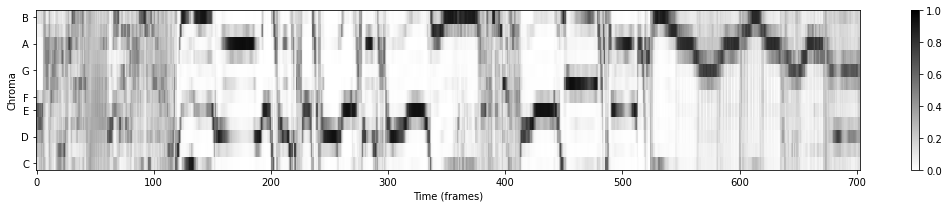
\includegraphics[width=\textwidth]{chromas/bo_cartero_trama.png}
    \end{figure}
    
\end{frame}

\begin{frame}{Cromagrama - Tuning}
    \textbf{Problema:}
    Los cromagramas son sensibles a pequeñas desafinaciones en la canción respecto a la escala de 440Hz.
    
    \vfill
    
    \textbf{Solución:} la librería librosa tiene funciones para la estimación de desafinación y la corrección. Funcionamiento:
    \begin{enumerate}
        \item Estima frecuencia fundamental en el tiempo (con STFT)
        \item Calcula la distancia a la nota en la escala más cercana para cada frame
        \item Mediante un histograma, toma la distancia con más ocurrencias como desvío
    \end{enumerate}
    
\end{frame}

\begin{frame}{Cromagrama - Tuning}
    \begin{figure}
        \begin{subfigure}{\textwidth}
        \centering
        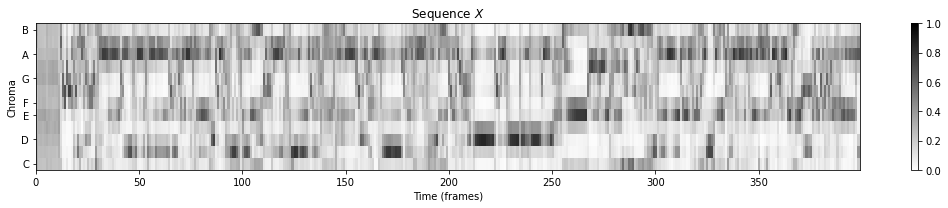
\includegraphics[width=\textwidth]{chromas/solo_un_rumor_sin.png}
        \label{fig:my_label}
        \end{subfigure}
        \vfill
        \begin{subfigure}{\textwidth}
        \centering
        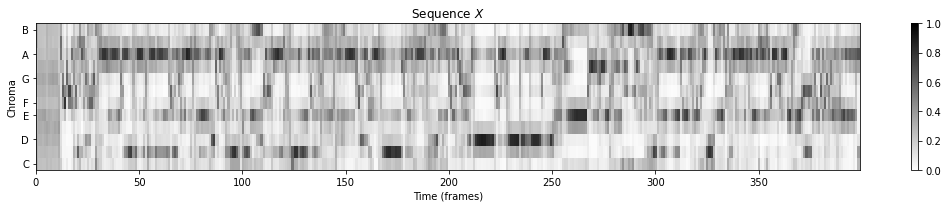
\includegraphics[width=\textwidth]{chromas/solo_un_rumor_tuning.png}
        \caption{Solo un rumor. Arriba sin tuning, abajo con tuning automático.}
        \label{fig:my_label}
        \end{subfigure}
    \end{figure}
\end{frame}

\begin{frame}{Cromagrama - Tone Shift}
    \textbf{Problema:} algo muy común en covers es cambiar la tonalidad de la canción para ajustarla a un nuevo cantante o estilo.
    \vfill
    \textbf{Solución:} Se estima el shift óptimo de uno de los croma que minimiza la distancia DTW. 
\end{frame}

\begin{frame}{Cromagrama - Normalización y compresión}
    \textbf{Problema:} Armónicos que aparecen con diferente intensidad. Además las notas se pueden tocar con distintas intensidades.
    \vfill
    \textbf{Solución:} Se aplica compresión logarítmica para acercar las amplitudes del cromagrama. Se aplica normalización para que todas las tramas tengan la misma energía y no se extinga tan rápidamente. 
\end{frame}

\begin{frame}{Cromagrama final}
\begin{itemize}
    \item Se siguió un tutorial de librosa para limpiar el cromagrama. 
    \begin{enumerate}
        \item Obtención de componentes armónicos con hpss. 
        \item Filtrado no local basado en vecinos mas cercanos.
        \item Eliminación de transitorios y discontinuidades horizontales con filtro de mediana. 
    \end{enumerate}
\end{itemize}
\begin{figure}[!h]
    \centering
    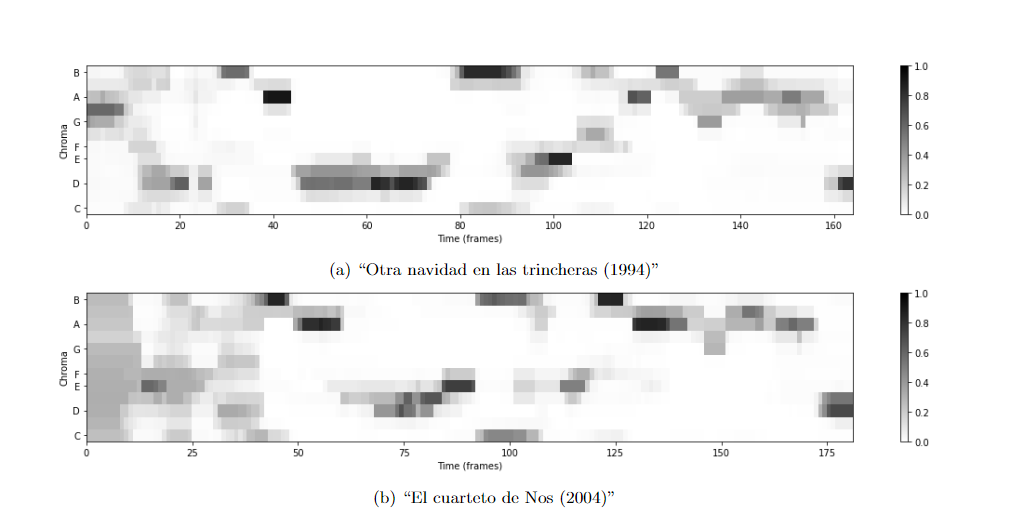
\includegraphics[width=0.8\textwidth]{chromas/pretty_cromas.png}
    \caption{Cromas finales en introducción de Bo cartero}
    \label{pretty_cromas}
\end{figure}
\end{frame}

%---------------------------------------------------------

\subsection{DTW}

\begin{frame}{DTW}
    El DTW es un algoritmo que permite cuantificar la similitud entre dos secuencias.
    \begin{itemize}
        \item Las secuencias no tienen por qué tener el mismo largo.
    \end{itemize}
    \vfill
    Un pseudocódigo del algoritmo es el siguiente:
    \begin{enumerate}
        \item se calcula la matriz de costo
        \item se calcula la matriz de costo acumulado
        \item se aplica backtracking para hallar el camino de menor costo
    \end{enumerate}
\end{frame}

\begin{frame}{DTW}
\begin{figure}
    \begin{subfigure}{0.49\textwidth}
        \centering
        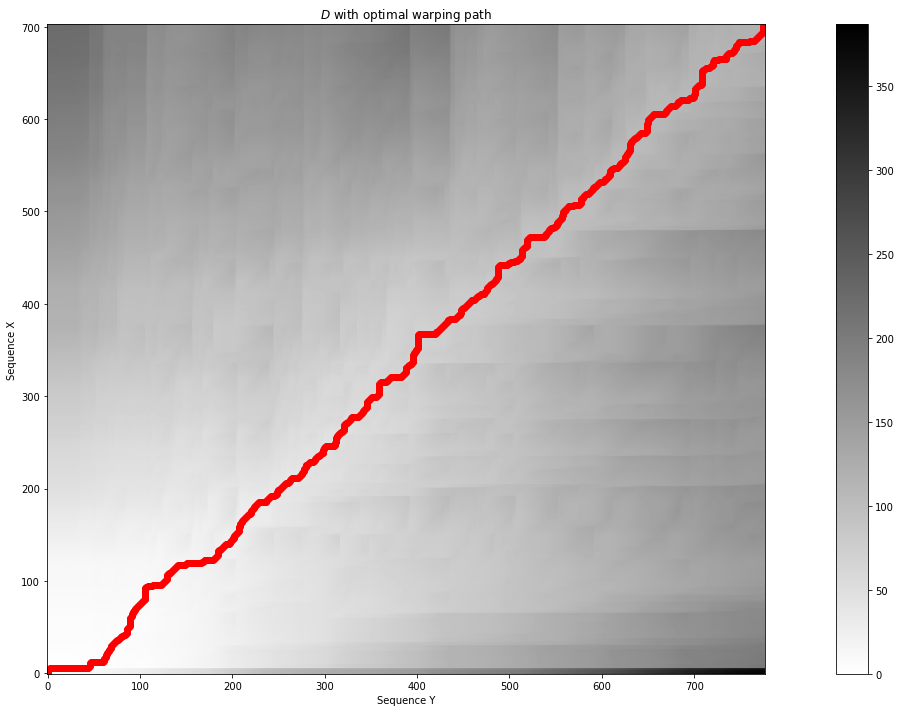
\includegraphics[width=\textwidth]{dtw_bo_cartero.png}
        \caption{path DTW para intro de bo cartero}
    \end{subfigure}
    \hfill
    \begin{subfigure}{0.49\textwidth}
        \centering
        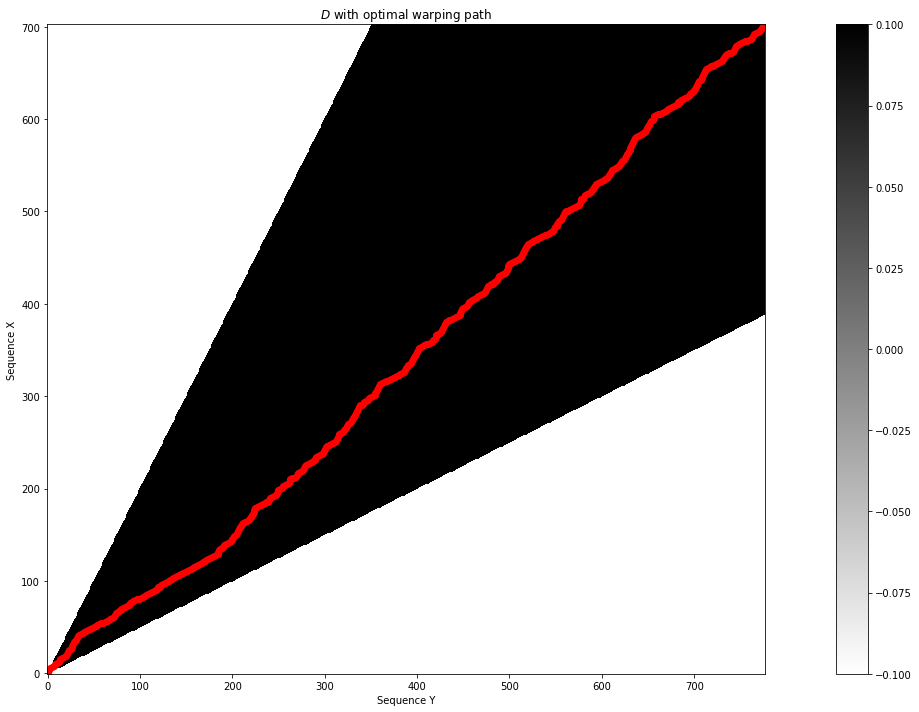
\includegraphics[width=\textwidth]{dtw_bo_cartero_step_size.png}
        \caption{step size $\{(1,2), (2,1), (1,1)\}$}
    \end{subfigure}
\end{figure}

\end{frame}

%---------------------------------------------------------
\subsection{Detector de covers}

\begin{frame}{Detector de covers}
\begin{itemize}
    \item Para fijar los parámetros del DTW se compararon todos los covers menos ``El puton del barrio'' y ``Me agarre el pitito con el cierre'' y con eso se cambio la funcion de costo, las restricciones sobre el camino y cambios en el step\_size.
    \item Se termino eligiendo la distancia coseno, $\{ (1,2), (2,1), (1,1) \}$ como step\_size (es decir estrictamente monótona creciente) y no se aplicaron restricciones globales.
    \item La distancia se normalizo respecto al largo del path para tener una independencia en cuanto a la relación entre el largo de las canciones.
\end{itemize}
\end{frame}

\begin{frame}{Detector de covers}
    \begin{figure}
        \centering
        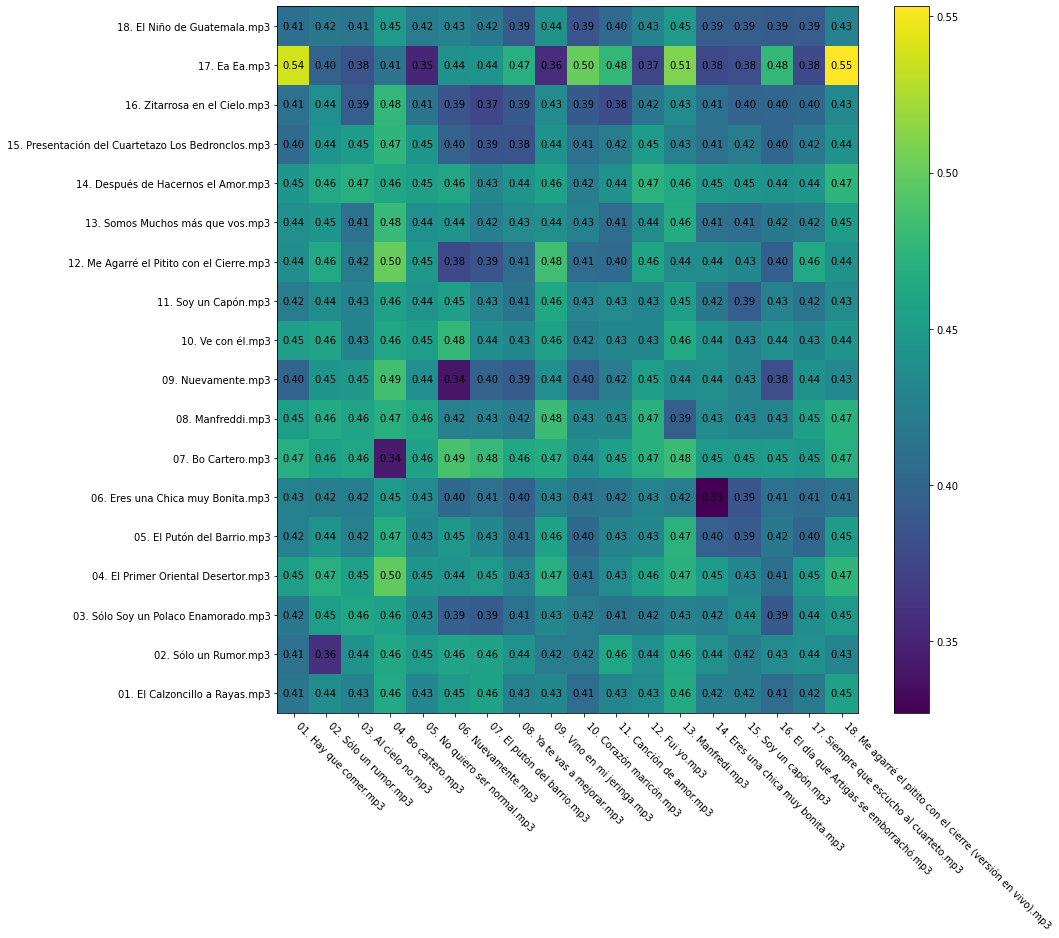
\includegraphics[width=0.8\textwidth]{chromas/matrix_all_vs_all.png}
    \end{figure}
    
\end{frame}




%---------------------------------------------------------
\section{Segunda etapa}
\subsection{Estudio de la cancion elegida}
\begin{frame}{Estudio de la canción elegida}
\begin{itemize}
    \item La canción elegida fue ``Bo cartero" dado que había sido detectada correctamente por el detector de covers. 
    \item Algunas diferencias encontradas son:
    \begin{enumerate}
        \item Diferencias en la velocidad de interpretación.
        \item Intensidad con la que se escuchan los instrumentos y la voz cantada.
        \item Diferencias en la sección instrumental.
        \item Diferentes palabras utilizadas en la ultima estrofa. 
    \end{enumerate}
\end{itemize}
\end{frame}

\subsection{Alineamiento}
\begin{frame}{Alineamiento}
\begin{itemize}
    \item Se usa la función hps\_tsm de libtsm. Esta función resuelve el problema de alineación temporal en los siguientes pasos.
    \begin{enumerate}
        \item Separación de componentes armónicos y percusivos con un filtro de mediana en el sentido vertical del espectrograma para los componentes percusivos y en el sentido horizontal para los armónicos. Esto es por que el phase vocoder pre supone una representación armónica que los percusivos no tienen.
        \item Phase vocoder basado en una función de deformacion (el path) para armónicos.
        \item WSOLA para percusivos, que es Waveform Similarity OverLap Add.
    \end{enumerate}
    \item Tambien se probo el notebook de la librería Synctoolbox que usa los DLNCO features (que dan mas precision temporal) y MrMsDTW que es un DTW de menor costo computacional. 
\end{itemize}
\end{frame}
\begin{frame}{Alineamiento}
\begin{itemize}
    \item Se debieron realizar algunas modificaciones al DTW que había sido optimizado para un problema de diferente naturaleza.
    \item Las modificaciones fueron:
    \begin{enumerate}
        \item Cambio de resolución en el calculo del cromagrama siguiendo como referencia el notebook de Synctoolbox.
        \item Eliminación de la limpieza del cromagrama. Especialmente la parte de solo obtener los componentes armónicos, dado que los percusivos al ser puntuales en el tiempo pueden ayudar a un mejor alineamiento.
        \item Asegurarse de que es un camino estrictamente creciente para evitar problemas de repetición.
    \end{enumerate}
\end{itemize}
\end{frame}

\begin{frame}{Alineamiento}
\begin{itemize}
    \item En primer lugar se realizo el alineamiento de la introducción para poder comparar la correspondencia temporal entre las señales en el tiempo y los espectrogramas luego de la alineación.
    \item El resultado auditivo esta en el siguiente \href{https://drive.google.com/file/d/1ENzDIU0i8SvjrMq9fPpBsoJTDvhX7c2h/view?usp=sharing}{link}.
    \item La correspondencia temporal de estas secuencias es 
       \begin{figure}
        \centering
        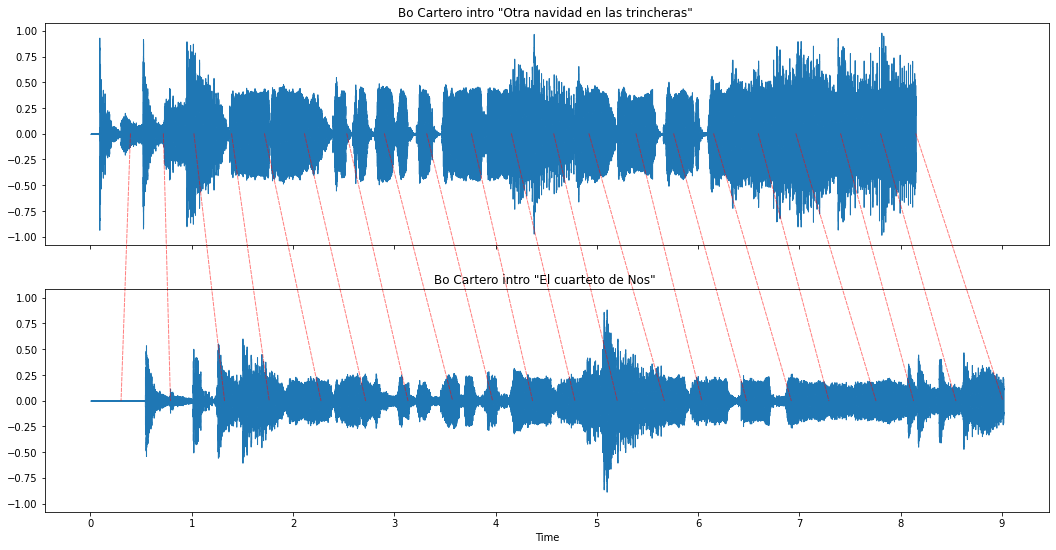
\includegraphics[width=0.8\textwidth]{alineamiento.png}
    \end{figure}
\end{itemize}
    
\end{frame}
\begin{frame}{Alineamiento}
  \begin{figure}
        \centering
        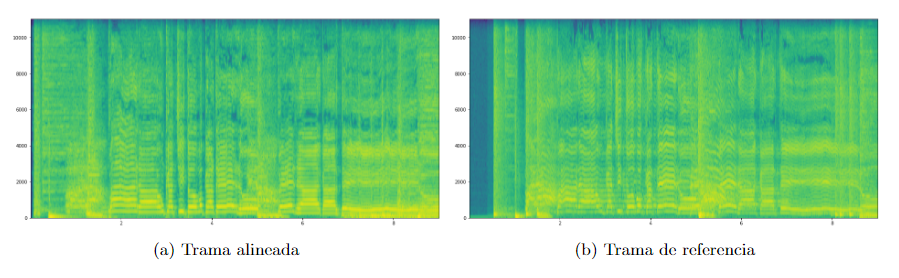
\includegraphics[width=1\textwidth]{espectrogramas.png}
    \end{figure}
\end{frame}
\begin{frame}{Alineamiento}
\begin{itemize}
    \item El alineamiento completo se puede escuchar en el siguiente \href{https://drive.google.com/file/d/1xiB5YNNIlJ8gaIPRDziwazqU-TdGHNDC/view?usp=sharing}{link}
    \item Auditivamente se escucha relativamente bien pero con algunos problemas.
    \item Las mayores diferencias se encuentran en los lugares donde se habían notado diferencias auditivas grandes, como lo es la parte instrumental y la ultima estrofa.
    \item La voz cantada es lo que tiene mejor sincronización, el acompañamiento por momentos también pero es mas propenso a desfasarse. 
    \end{itemize}
\end{frame}
\begin{frame}{Métricas de desempeño}
\begin{itemize}
    \item Para evaluar de manera objetiva el alineamiento se propone hacer una estimación del beat. Para eso se usa la función de librosa que resuelve el problema en tres pasos
    \begin{enumerate}
        \item Encuentra la intensidad con la cual comienza cada nota (onset) 
        \item Hace una estimación del tempo con la correlación de la intensidad calculada.
        \item Elige los picos de la intensidad que sean consistentes con el tempo estimado.
    \end{enumerate}
    \item La métrica de desempeño consiste en 
    \begin{enumerate}
        \item Calcular los beats de los canales.
        \item Hacer la resta y graficar eso en un histograma.
        \item Tomar el rango de mayor ocurrencia como métrica.
        \item Comparar con un umbral pre-establecido.
    \end{enumerate}
\end{itemize}
    
\end{frame}
\begin{frame}{Métricas de desempeño}
\begin{itemize}
    \item Si se establece como umbral 100ms, se puede considerar un buen alineamiento. 
\end{itemize}
  \begin{figure}
        \centering
        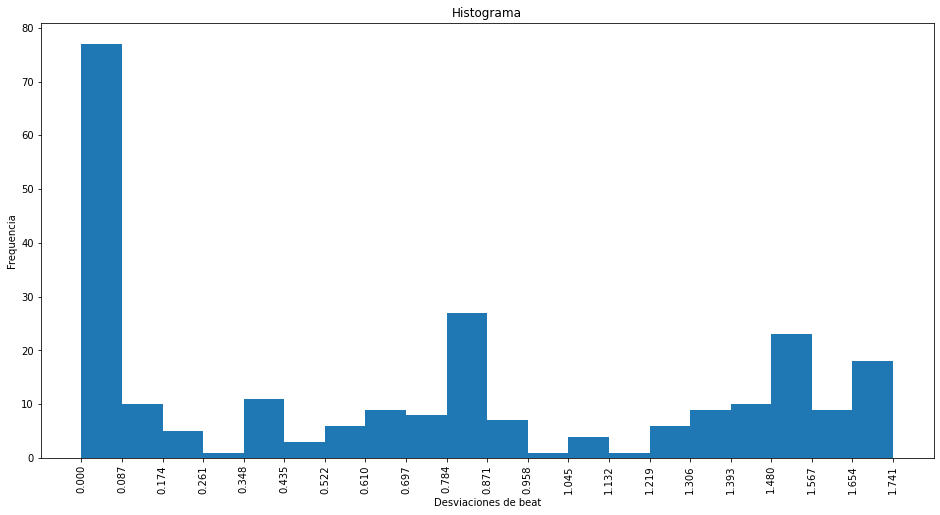
\includegraphics[width=1\textwidth]{histograma.png}
    \end{figure}
    
\end{frame}
\section{Conclusiones}
\begin{frame}{Conclusiones}
\begin{itemize}
    \item Se logro implementar un detector de covers con un desempeño satisfactorio y bajando el costo computacional se logro hacer la comparación de todas las canciones contra todas.
    \item Se pudo evaluar el impacto de los diversos parámetros a la hora de alinear secuencias.
    \item Se estableció una manera objetiva de evaluar el alineamiento que da lugar a muchas mejoras como lo es tener en cuenta mas picos, etc.
    
\end{itemize}
    
\end{frame}
\end{document}